\section{UEQ}
\label{sec:ueqs}

Nachfolgend finden sich die im Rahmen der Evaluation durch die Testkandidaten ausgefüllten Fragebögen (Abbildungen \ref{fig:UEQ1} - \ref{fig:UEQ5}).

\begin{figure}[h!]
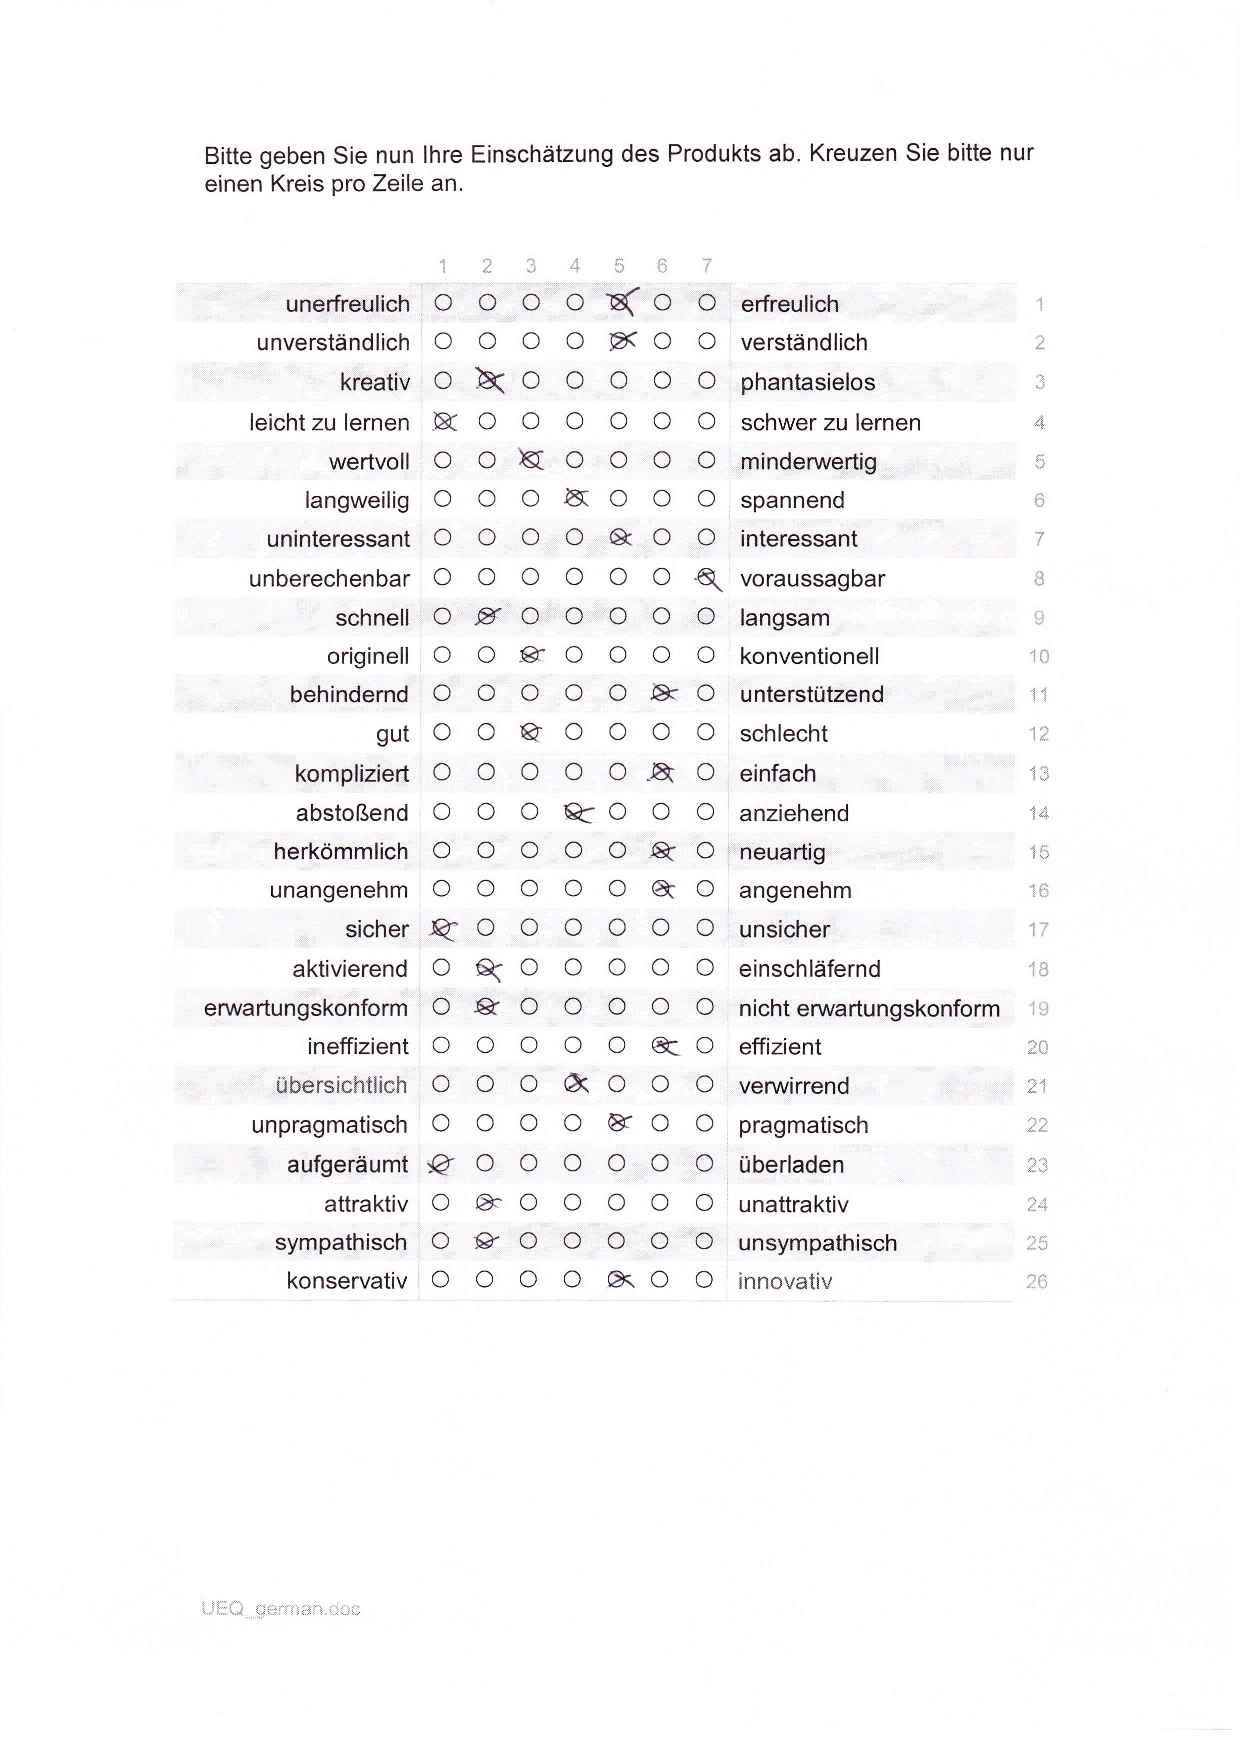
\includegraphics[width=0.77\textwidth,center]{UEQ1.pdf}
\caption{\label{fig:UEQ1}Fragebogen Testkandidat Nr. 1}
\end{figure}
\begin{figure}[h!]
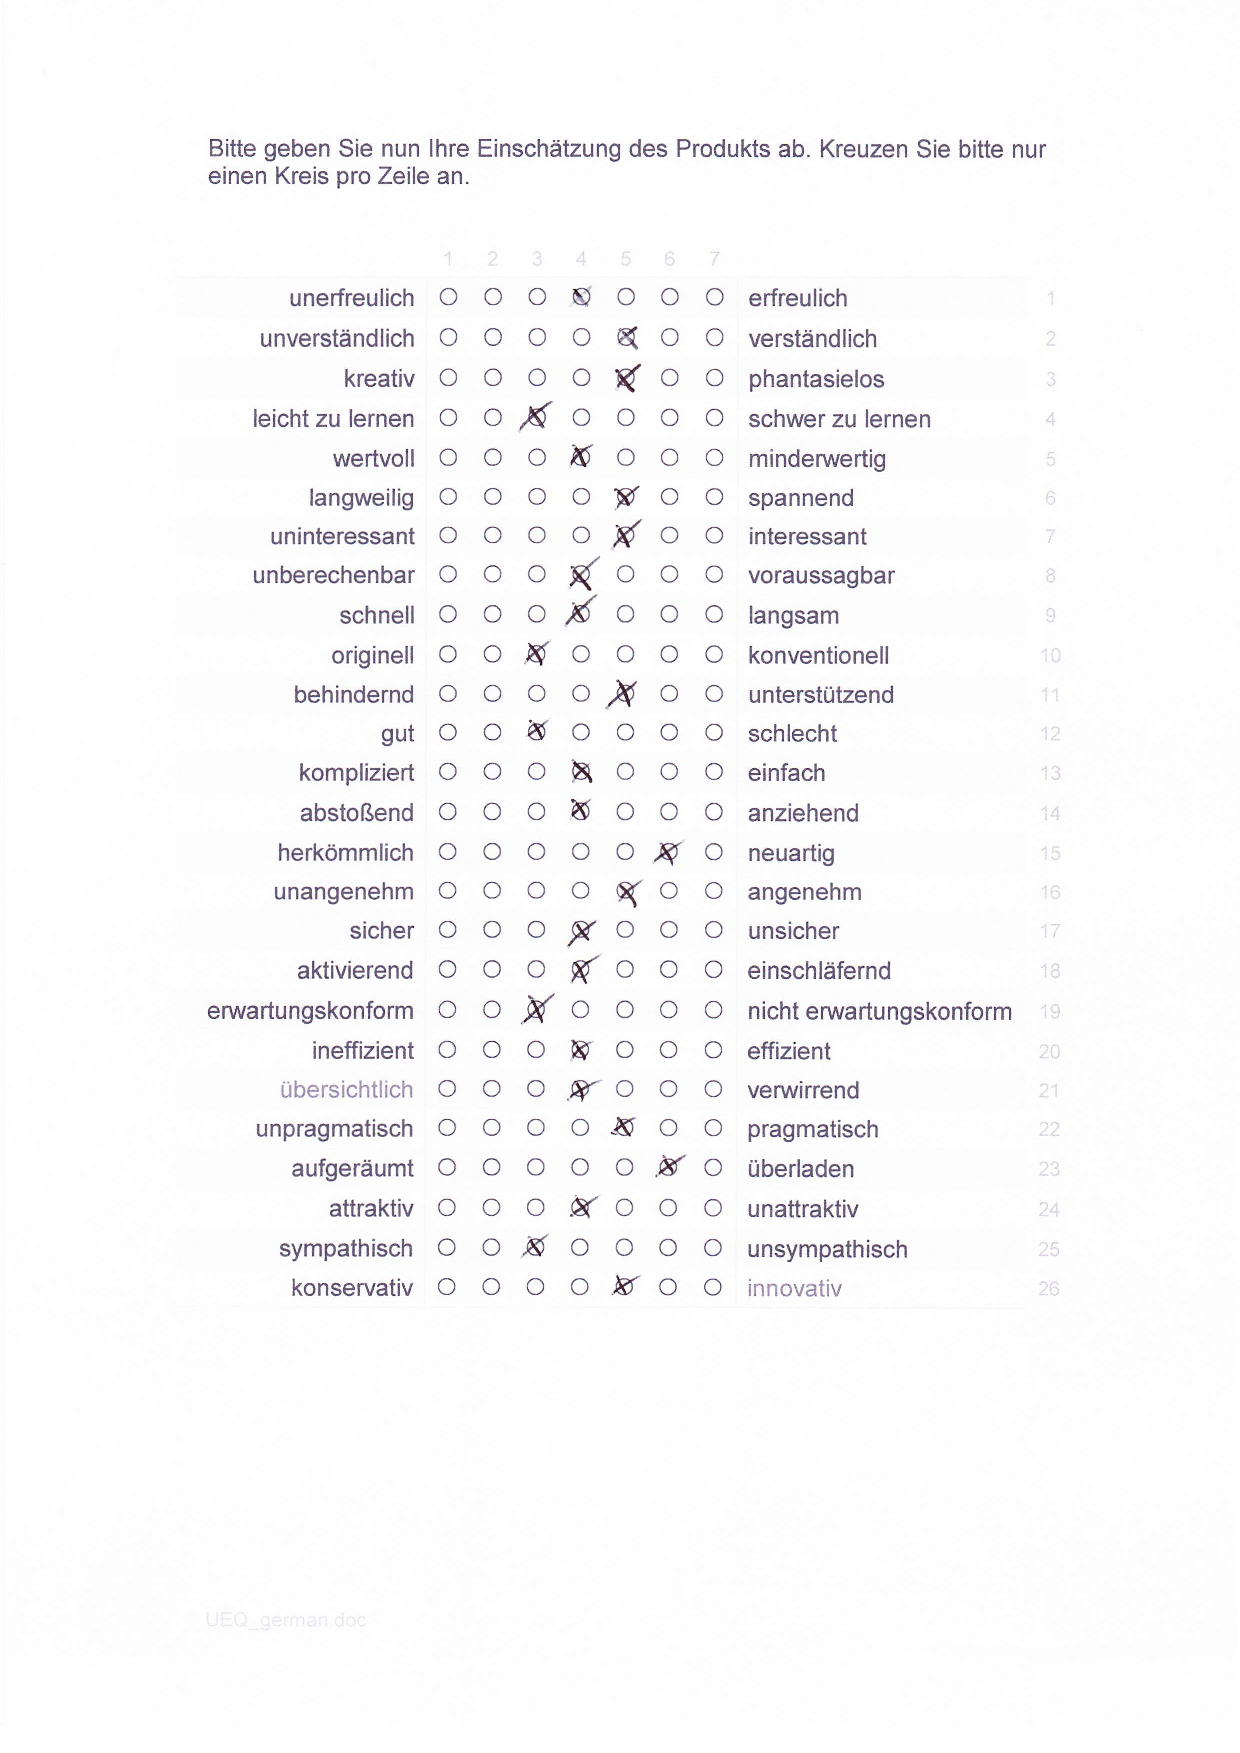
\includegraphics[width=0.77\textwidth,center]{UEQ2.pdf}
\caption{\label{fig:UEQ2}Fragebogen Testkandidat Nr. 2}
\end{figure}
\begin{figure}[h!]
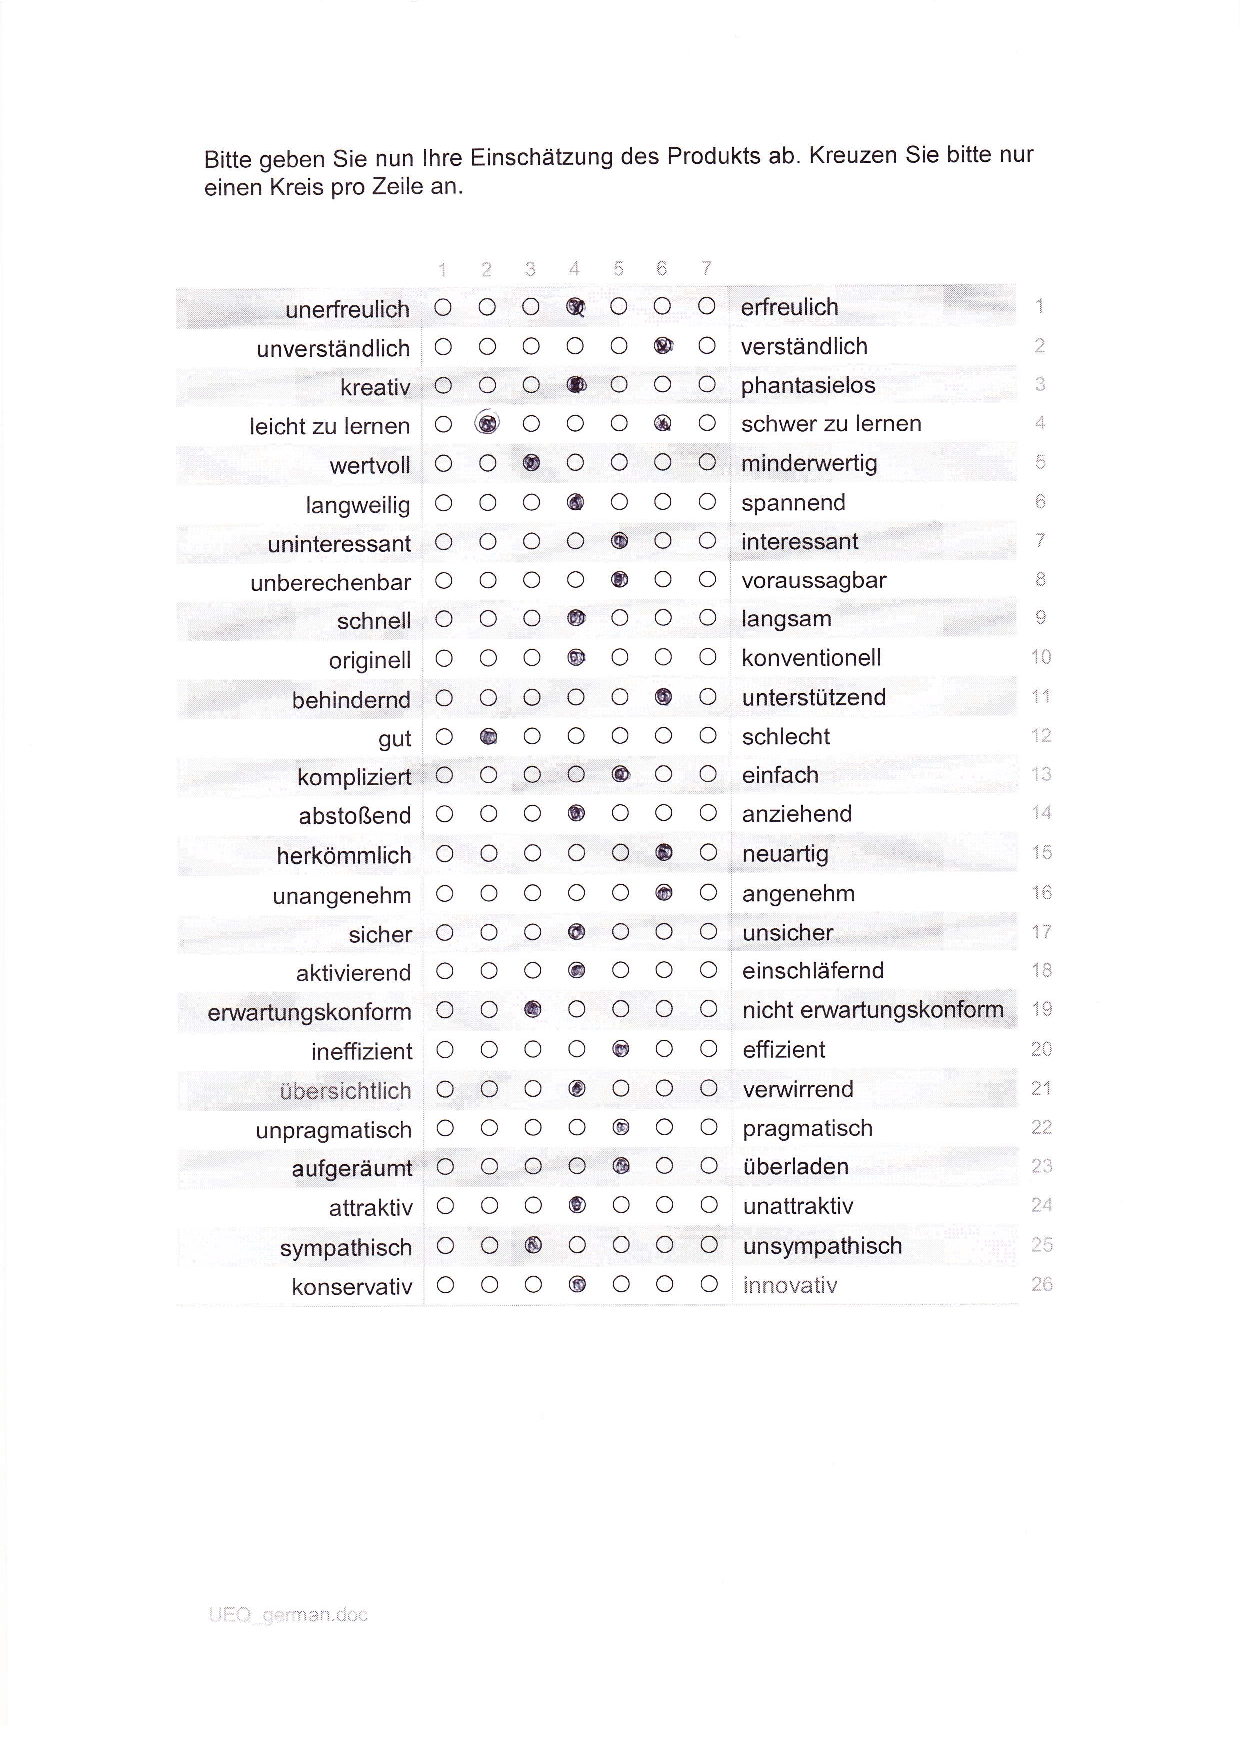
\includegraphics[width=0.77\textwidth,center]{UEQ3.pdf}
\caption{\label{fig:UEQ3}Fragebogen Testkandidat Nr. 3}
\end{figure}
\begin{figure}[h!]
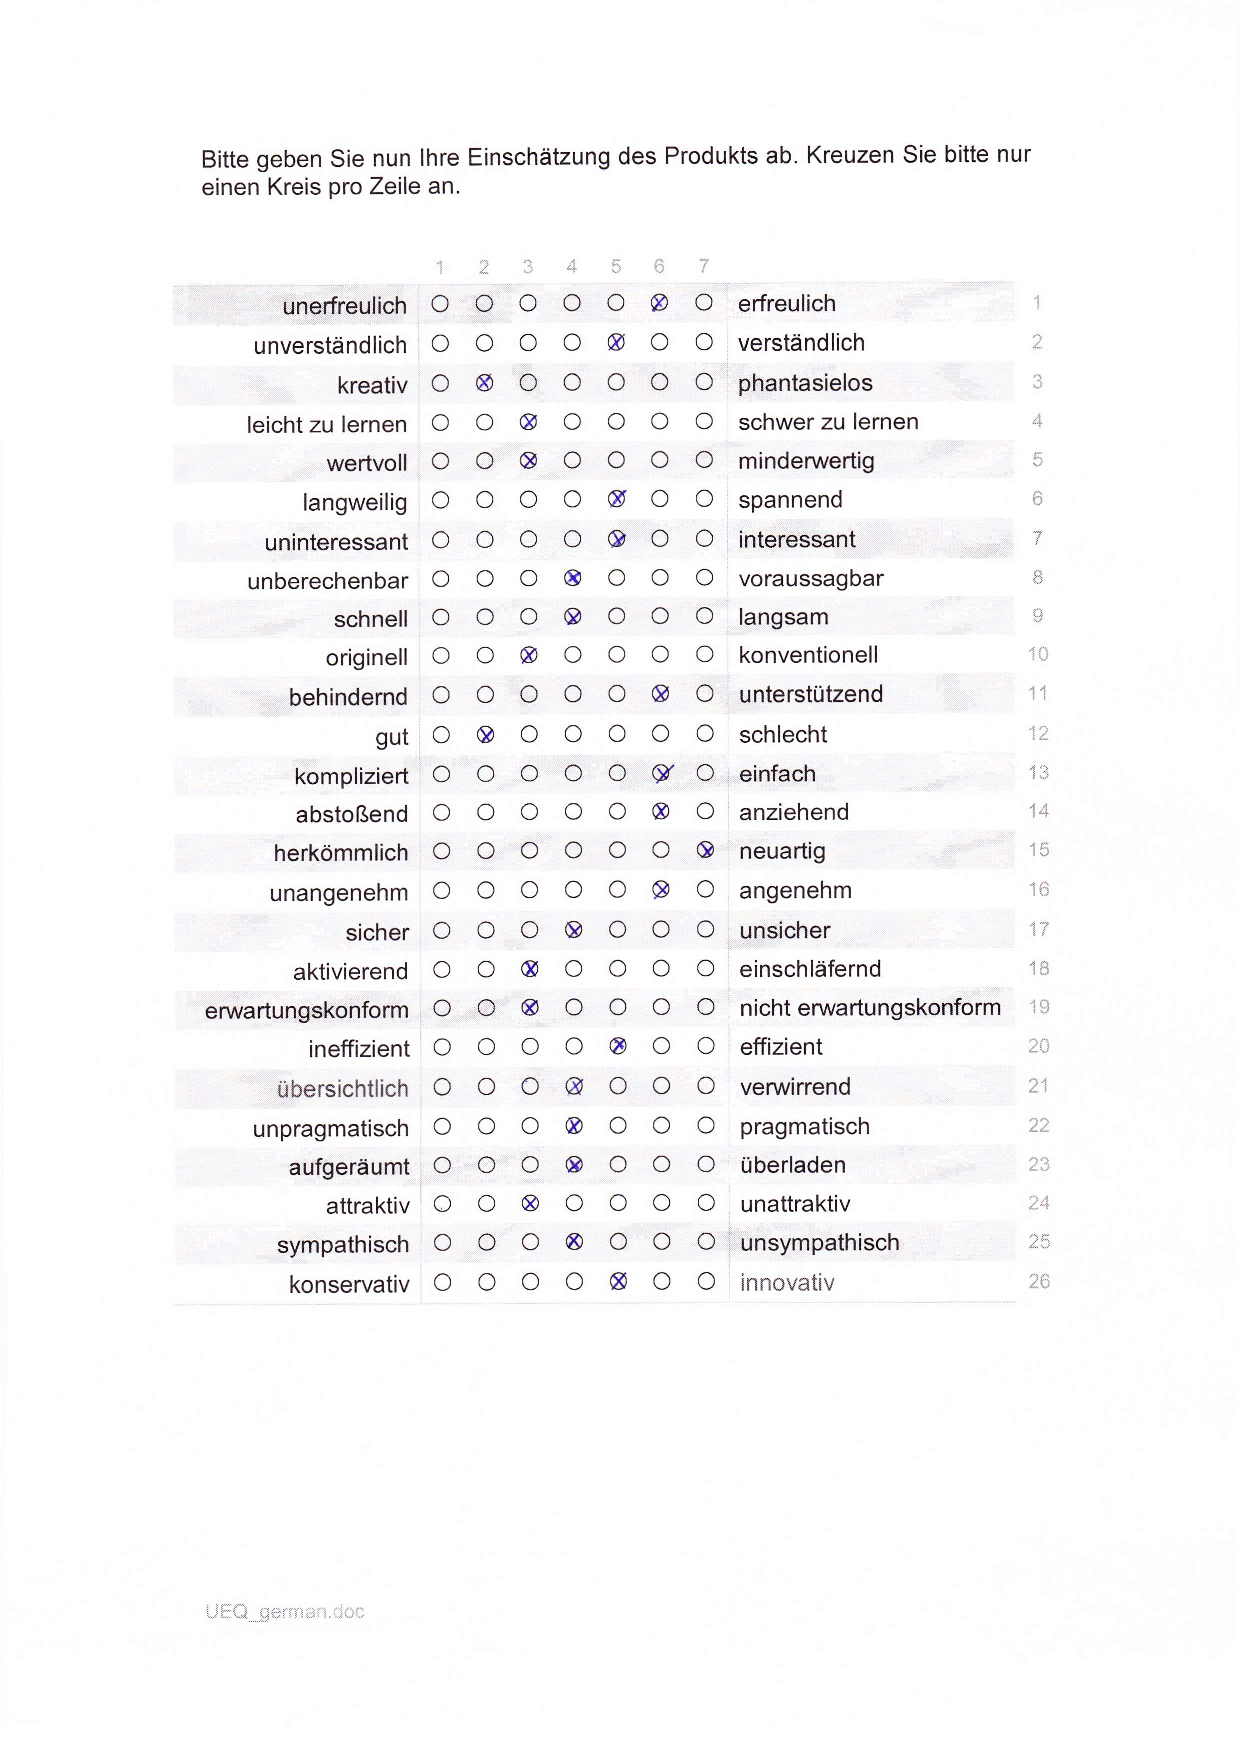
\includegraphics[width=0.77\textwidth,center]{UEQ4.pdf}
\caption{\label{fig:UEQ4}Fragebogen Testkandidat Nr. 4}
\end{figure}
\begin{figure}[h!]
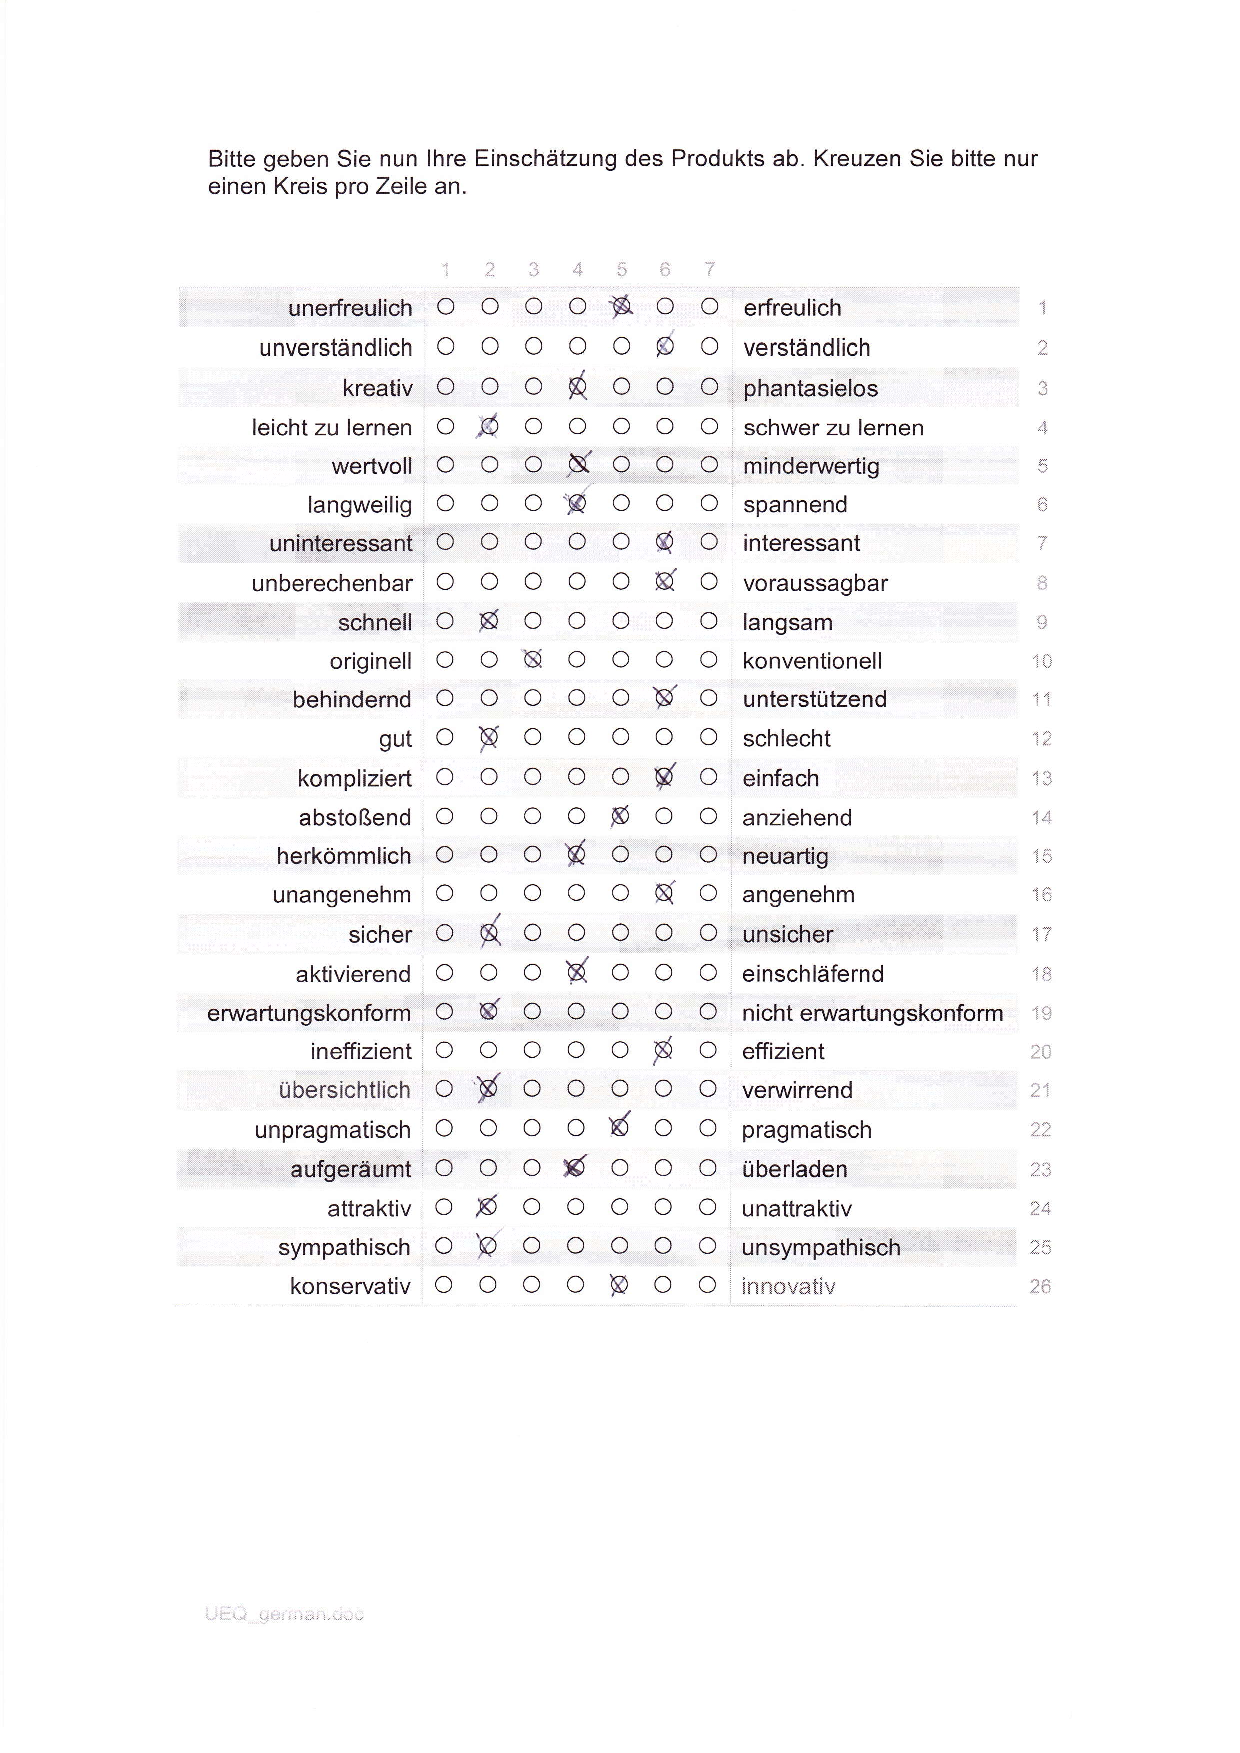
\includegraphics[width=0.77\textwidth,center]{UEQ5.pdf}
\caption{\label{fig:UEQ5}Fragebogen Testkandidat Nr. 5}
\end{figure}

\FloatBarrier

\section{Gesprächsnotizen}
\label{sec:gesprächsnotizen}

Nach dem Ausfüllen des Fragebogens fand ein Gespräch mit den Testkandidaten statt, in welchem diese Wünsche bezüglich funktionaler Erweiterungen des Plugins anbringen konnten. Die Vorschlage wurden stichpunktartig festgehalten (vgl. Tabellen \ref{tab:gesprächsnotizen1} - \ref{tab:gesprächsnotizen5}).

\begin{table}[!ht]
\centering
\def\arraystretch{1.4}
%\resizebox{\textwidth}{!}
    \caption{Gesprächsnotizen Testkandidat Nr. 1}
\label{tab:gesprächsnotizen1}
\end{table}

\begin{table}[!ht]
\centering
\def\arraystretch{1.4}
%\resizebox{\textwidth}{!}
    \caption{Gesprächsnotizen Testkandidat Nr. 2}
\label{tab:gesprächsnotizen2}
\end{table}

\begin{table}[!ht]
\centering
\def\arraystretch{1.4}
%\resizebox{\textwidth}{!}
    \caption{Gesprächsnotizen Testkandidat Nr. 3}
\label{tab:gesprächsnotizen3}
\end{table}

\begin{table}[!ht]
\centering
\def\arraystretch{1.4}
%\resizebox{\textwidth}{!}
    \caption{Gesprächsnotizen Testkandidat Nr. 4}
\label{tab:gesprächsnotizen4}
\end{table}

\begin{table}[!ht]
\centering
\def\arraystretch{1.4}
%\resizebox{\textwidth}{!}
    \caption{Gesprächsnotizen Testkandidat Nr. 5}
\label{tab:gesprächsnotizen5}
\end{table}

